%%
%% getstart.tex -- Flight Gear documentation: Installation and Getting Started
%% Chapter file
%%
%% Written by Michael Basler, started September 1998.
%%
%% Copyright (C) 1999 Michael Basler (pmb@knUUt.de)
%%
%%
%% This program is free software; you can redistribute it and/or
%% modify it under the terms of the GNU General Public License as
%% published by the Free Software Foundation; either version 2 of the
%% License, or (at your option) any later version.
%%
%% This program is distributed in the hope that it will be useful, but
%% WITHOUT ANY WARRANTY; without even the implied warranty of
%% MERCHANTABILITY or FITNESS FOR A PARTICULAR PURPOSE.  See the GNU
%% General Public License for more details.
%%
%% You should have received a copy of the GNU General Public License
%% along with this program; if not, write to the Free Software
%% Foundation, Inc., 675 Mass Ave, Cambridge, MA 02139, USA.
%%
%% $Id: getstart.tex,v 0.12 1999/03/07 michael

%%%%%%%%%%%%%%%%%%%%%%%%%%%%%%%%%%%%%%%%%%%%%%%%%%%%%%%%%%%%%%%%%%%%%%%%%%%%%%%%%%%%%%%%%%%%%%%%%
\chapter{Flight: Keystrokes,\index{keystrokes} the \Index{HUD}  and all that\label{flight}}
%%%%%%%%%%%%%%%%%%%%%%%%%%%%%%%%%%%%%%%%%%%%%%%%%%%%%%%%%%%%%%%%%%%%%%%%%%%%%%%%%%%%%%%%%%%%%%%%%
\markboth{\thechapter.\hspace*{1mm}
FLIGHT}{\thesection\hspace*{1mm} KEYBOARD COMMANDS}

\section{Keyboard commands}

At present, support for using a \Index{joystick} or \Index{yoke}
is just in its early stages. It may or may not work -- just try
it! In any case, you can use \Index{keyboard commands} instead.
For proper controlling via keyboard (i) the
\texttt{\Index{NumLock}} key must be switched on (ii) the
\FlightGear window must have focus (if not, click with the mouse
on the graphics window).

After activating \texttt{NumLock} the following \Index{keyboard
commands} should work:
\medskip

\noindent
 Tab.\,1: \textit{Main \Index{keyboard commands} for \FlightGear}.
\medskip

\centerline{
\begin{tabular}{|l|l|}\hline
 Key                       &  Action\\\hline
 Pg Up/Pg Dn               &  Throttle\\
 Left Arrow/Right Arrow    &  Aileron\\
 Up Arrow/Down Arrow       &  Elevator\\
 Ins/Enter                 &  Rudder\\
 5                         &  Center aileron/elevator/rudder\\
 Home/End                  &  Elevator trim\\\hline
\end{tabular}
}
\vskip5mm

For changing views you have to de-activate \texttt{NumLock}. Now
\texttt{Shift} + $<$\texttt{Numeric Keypad Key}$>$ changes the
view as follows:
 \eject

\noindent
 Tab.\,2: \textit{View directions\index{view directions}
accessible after de-activating \texttt{NumLock}.}
\medskip

\centerline{
\begin{tabular}{|c|l|}\hline
 Numeric Key  &  View direction\\\hline
    Shift-8 & forward\\
    Shift-7 & left/forward\\
    Shift-4 & left\\
    Shift-1 & left/back\\
    Shift-2 & back\\
    Shift-3 & right/back\\
    Shift-6 & right\\
    Shift-9 & right/forward\\\hline
\end{tabular}
}
\vskip5mm

Moreover, the \Index{autopilot} is controlled via the following
controls:
\medskip

\noindent
 Tab.\,3: \textit{Autopilot controls.\index{autopilot controls}}
\medskip

\centerline{
\begin{tabular}{|l|l|}\hline
 Key               &         Action\\\hline
    Ctrl + A      &         Altitude hold toggle on/off\\
    Ctrl + H      &         Heading hold toggle on/off\\
    Ctrl + S      &         Autothrottle toggle on/off\\
    Ctrl + T      &         Terrain follow toggle on/off\\\hline
\end{tabular}
}
\medskip

The last one is especially interesting as it makes your
\Index{Navion} behave like a cruise missile.

Besides these basic keys there are some more special ones; most of
these you'll probably not want to try during your first flight:
\medskip

\noindent Tab.\,4: \textit{More control commands.}
\medskip

\centerline{
\begin{tabular}{|l|l|}\hline
Key                       &  Action\\\hline
     H/h    & Change color  of HUD/toggle HUD off forward/backward      \\
   i/I     & Minimize/maximize HUD              \\
   m/M  & Change time offset (warp) used by t/T forward/backward              \\
   t/T  & Time speed up/slow down  forward/backward            \\
   x/X  & Zoom in/out\\
   z/Z &  Change visibility (fog)  forward/backward \\
   b & Toggle brakes on/off\\
   p & Toggle pause on/off\\
   W & Toggle fullscreen mode on/off (Mesa/3dfx/Glide only)\\
   F8 & Toggle fog on/off\\
   F9 & Toggle texturing on/off\\
   F10 & Toggle menu on/off\\
   ESC & Exit program\\\hline
\end{tabular}
}
\medskip

\section{The head up display}

At present, the main instrument for controlling the plane is the
\Index{HUD}  (\textbf{H}ead \textbf{U}p \textbf{D}isplay
\index{head up display}, see Fig.\,1). Neither are \Index{HUD}s
used in usual general aviation planes nor in civilian ones. Rather
they belong to the equipment of modern military jets. However, in
view of the fact that the \Index{panel} is still in the early
stages of development the \Index{HUD} is the main instrument for
controlling the plane for now. Besides, it might be easier to fly
using this one than exploiting a \Index{panel} and several of the
real pilots might prefer it because of combining the readouts of
critical parameters with an outside view onto the real world.
(Several \Index{Cessna} pilots might love to have one, but
technology is simply too expensive for implementing HUDs in
general aviation aircrafts.)
 \medskip

 \centerline{
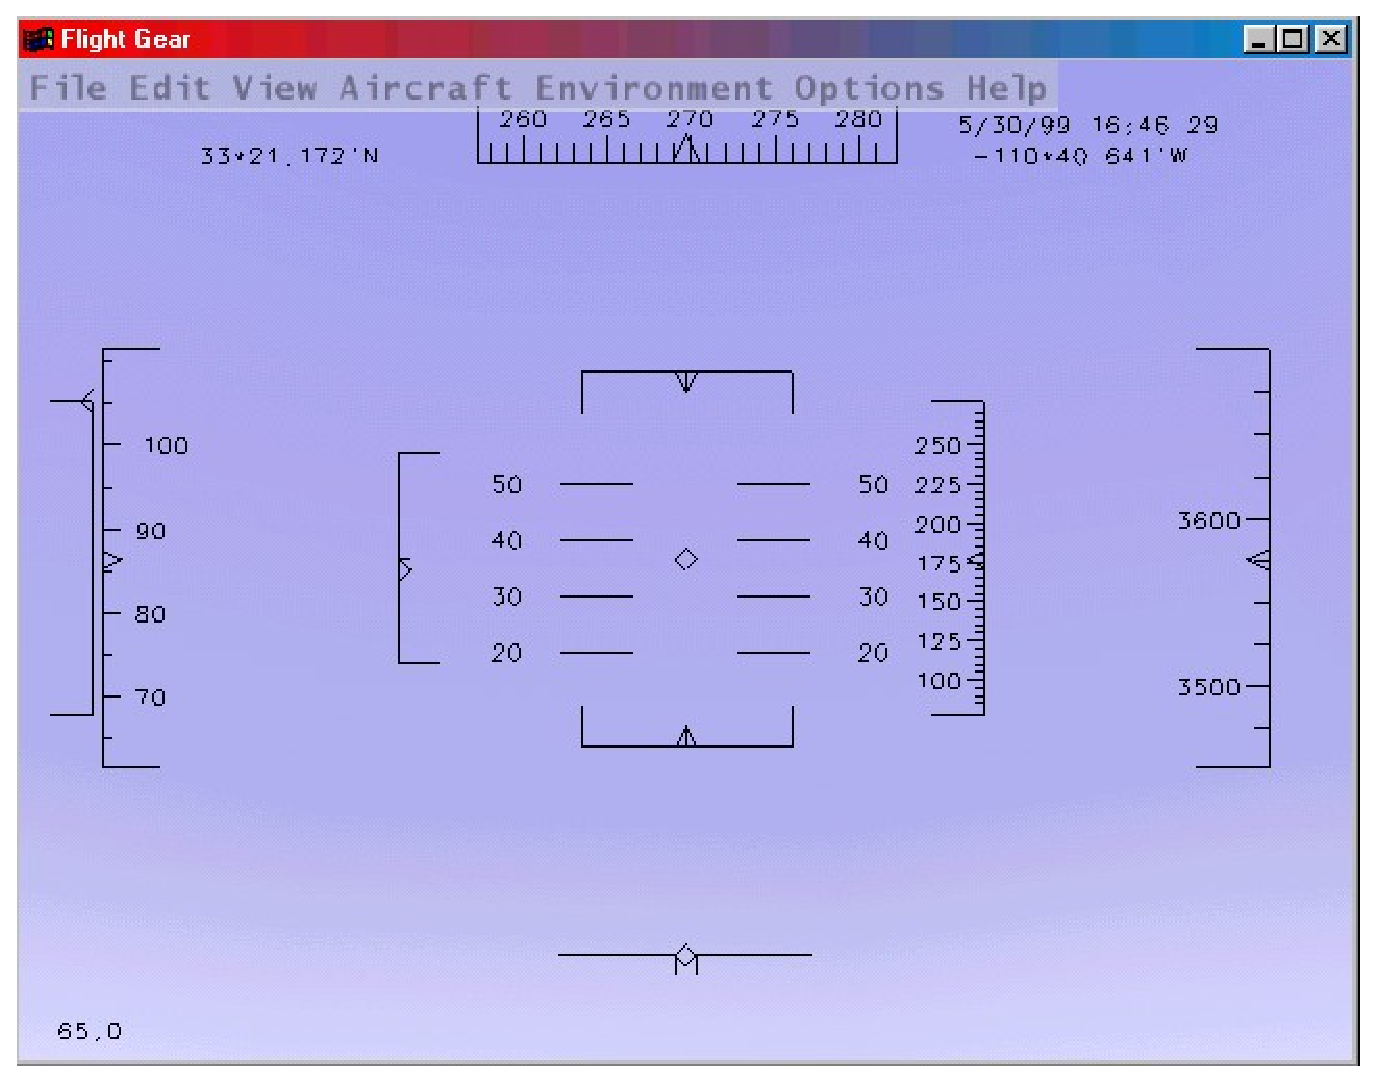
\includegraphics[clip,width=12.5cm]{hud.eps}
}

 \noindent
Fig.\,3: \textit{The HUD, or head up display, as the present main
\FlightGear instrument.}
\medskip

The most important information for navigating, i.\,e.
\Index{throttle}, \Index{elevation}, \Index{aileron} can be found
on the r.h.s of the \Index{HUD}. These are just given on a scale
between 0 and 1. Above these you find the \Index{AOA}
(\Index{angle of attack}; the angle between the wings and the
relative wind i.\,e. the direction of airflow), the
\Index{heading} given in degrees, and the \Index{sideslip}.

On the left hand side you find the \Index{speed} in kts and the
\Index{roll} given in degrees. You may recall the \Index{Navion}
taking off at a speed of 100 kts. Still further left you find the
\Index{FOV} (= \Index{field of view}) in degrees.
Zooming\index{zoom} in and out with the x/X keys changes this one.
The value below that, the \Index{number of triangles} rendered is
usually not of importance for you as a pilot (and can be switched
off via a corresponding startup option). Below you find the
\Index{frame rate}, displaying the frames per second.

Besides these figures, most of the flight parameters and flight
characteristics are displayed graphically in the upper half of the
screen. In the center you find the \Index{pitch indicator} (in
degrees) with the \Index{aileron indicator} above and the
\Index{rudder indicator} below. A corresponding readoff for the
elevation\index{elevation indicator} can be found to the left of
the pitch scale. Below the \Index{pitch indicator} you will find a
simple \Index{turn indicator}.

There are two scales further left: The inner one displays the
\Index{speed} (in kts) while the outer one gives the
\Index{vertical speed} (\Index{climb/sink rate}). The two scales
on the r.h.s display your \Index{height}, i.\,e. the left of it
shows the height above ground while the right of it gives that
above zero, both being displayed in feet.

Based on these keystrokes and the HUD you should be able to
properly control the plane. Try it! The functions already
implemented are completely sufficient for even doing complicated
manoeuvres.

In addition, \FlightGear has a rudimentary menu which, however, is
not yet working. If you're done and are about to leave the plane,
just hit the ESC key to exit the program.

If you are looking for some interesting places to discover with
\FlightGear (which may or may not require downloading additional
scenery) you may want to check

 \web{http://www.flightgear.org/Downloads/Places}.

%% Revision 0.00  1998/09/08  michael
%% Initial revision for version 0.53.
%% Revision 0.01  1998/09/20  michael
%% several extensions and corrections, added Fig.1.
%% revision 0.10  1998/10/01  michael
%% final proofreading for release
%% revision 0.11  1998/11/01  michael
%% Complete revision of keyborad controls, interesting places
%% revision 0.12  1999/03/07  michael
%% Corrected rudder key
